%%%%%%%%%%%%%%%%%%%%%%%%%%%%%%%%%%%%%%%%%
% baposter Landscape Poster
% LaTeX Template
% Version 1.0 (11/06/13)
%
% baposter Class Created by:
% Brian Amberg (baposter@brian-amberg.de)
%
% This template has been downloaded from:
% http://www.LaTeXTemplates.com
%
% License:
% CC BY-NC-SA 3.0 (http://creativecommons.org/licenses/by-nc-sa/3.0/)
%
%%%%%%%%%%%%%%%%%%%%%%%%%%%%%%%%%%%%%%%%%

%----------------------------------------------------------------------------------------
%	PACKAGES AND OTHER DOCUMENT CONFIGURATIONS
%----------------------------------------------------------------------------------------

\documentclass[landscape,a0paper,fontscale=0.285]{baposter} % Adjust the font scale/size here

\usepackage{graphicx} % Required for including images
\graphicspath{{figures/}} % Directory in which figures are stored

\usepackage{amsmath} % For typesetting math
\usepackage{amssymb} % Adds new symbols to be used in math mode

\usepackage{booktabs} % Top and bottom rules for tables
\usepackage{enumitem} % Used to reduce itemize/enumerate spacing
\usepackage{palatino} % Use the Palatino font
\usepackage[font=small,labelfont=bf]{caption} % Required for specifying captions to tables and figures

\usepackage{multicol} % Required for multiple columns
\setlength{\columnsep}{1.5em} % Slightly increase the space between columns
\setlength{\columnseprule}{0mm} % No horizontal rule between columns

\usepackage{tikz} % Required for flow chart
\usetikzlibrary{shapes,arrows} % Tikz libraries required for the flow chart in the template

\newcommand{\compresslist}{ % Define a command to reduce spacing within itemize/enumerate environments, this is used right after \begin{itemize} or \begin{enumerate}
\setlength{\itemsep}{1pt}
\setlength{\parskip}{0pt}
\setlength{\parsep}{0pt}
}

\definecolor{lightblue}{rgb}{0.145,0.6666,1} % Defines the color used for content box headers

\begin{document}

\begin{poster}
{
headerborder=closed, % Adds a border around the header of content boxes
colspacing=1em, % Column spacing
bgColorOne=white, % Background color for the gradient on the left side of the poster
bgColorTwo=white, % Background color for the gradient on the right side of the poster
borderColor=lightblue, % Border color
headerColorOne=black, % Background color for the header in the content boxes (left side)
headerColorTwo=lightblue, % Background color for the header in the content boxes (right side)
headerFontColor=white, % Text color for the header text in the content boxes
boxColorOne=white, % Background color of the content boxes
textborder=roundedleft, % Format of the border around content boxes, can be: none, bars, coils, triangles, rectangle, rounded, roundedsmall, roundedright or faded
eyecatcher=true, % Set to false for ignoring the left logo in the title and move the title left
headerheight=0.1\textheight, % Height of the header
headershape=roundedright, % Specify the rounded corner in the content box headers, can be: rectangle, small-rounded, roundedright, roundedleft or rounded
headerfont=\Large\bf\textsc, % Large, bold and sans serif font in the headers of content boxes
%textfont={\setlength{\parindent}{1.5em}}, % Uncomment for paragraph indentation
linewidth=2pt % Width of the border lines around content boxes
}
%----------------------------------------------------------------------------------------
%	TITLE SECTION 
%----------------------------------------------------------------------------------------
%
{
\includegraphics[height=6em]{ruet.png}} % First university/lab logo on the left
{\bf\textsc{Target Class Oriented Subspace Detection for Effective Hyperspectral Image Classification}\vspace{0.1em}} % Poster title
{\textsc{\{ Md. Tanvir Ahmed, Md. Ali Hossain and Md. Al Mamun \} \hspace{12pt} Department of Computer Science \& Engineering, Rajshahi University of Engineering \& Technology}} % Author names and institution
{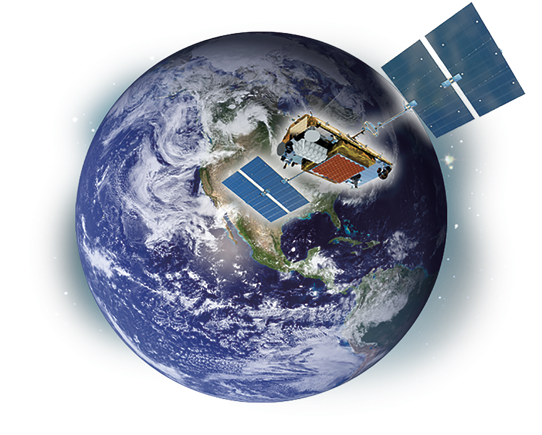
\includegraphics[height=6em]{sattelite.png}} % Second university/lab logo on the right

%----------------------------------------------------------------------------------------
%	OBJECTIVES
%----------------------------------------------------------------------------------------

\headerbox{Objectives}{name=objectives,column=0,row=0}{

To Achieve high classification accuracy in hyperspectral image classification.We proposed a target class oriented feature reduction method which incorporates the normalized Mutual Information (NMI) over PCA images to maximize the relevance of the selected subspace.  

\begin{enumerate}\compresslist
\item Ground object detection
\item Achive high classification accuracy
\item Minimize curse of dimensionality problems
\end{enumerate}

\vspace{0.3em} % When there are two boxes, some whitespace may need to be added if the one on the right has more content
}

%----------------------------------------------------------------------------------------
%	INTRODUCTION
%----------------------------------------------------------------------------------------

\headerbox{Introduction}{name=introduction,column=1,row=0,bottomaligned=objectives}{

In recent years, the hyperspectral image sensor has developed into one of the most powerful and fastest growing technologies in the area of remote sensing. This sensors provides data cube which contains rich information for wide range of application including effective land cover detection and classification. But this large data presents some challenges while classifying into constituesnt objects.We proposed a method called TCOSD to overcome the challenges while identifying one ground object at a time e.g. forest. 

\vspace{0.3em} 
}

%----------------------------------------------------------------------------------------
%	EXPERIMENTAL DATASET
%----------------------------------------------------------------------------------------

\headerbox{Experimental Dataset}{name=results,column=2,span=2,row=0}{

\begin{multicols}{2}
	
\begin{center}
	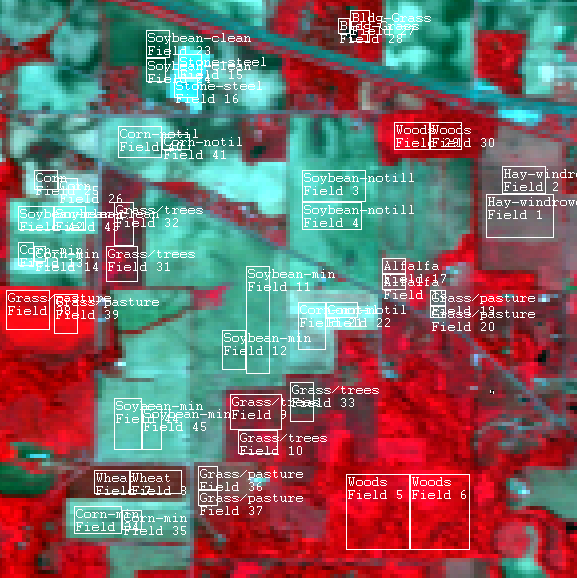
\includegraphics[width=.98\linewidth]{Dataset.png}
	\captionof{figure}{AVIRIS 92AV3C Dataset}
\end{center}
The Indian Pines scene contains
two-thirds agriculture, and one-third forest or other natural perennial vegetation.
\begin{center}
	\begin{tabular}{|l|l|l|}
		\hline
		Class name & Train & Test\\ \hline
		Hay-windrowed & 187 & 77\\ \hline
		Soybean-notil & 128 & 105\\ \hline
		Woods & 367 & 341\\ \hline
		Wheat & 54 & 78\\ \hline
		Grass/trees & 249 & 115\\ \hline
		Soybean-min & 253 & 115\\ \hline
		Corn-min & 253 & 115\\ \hline
		Stone-steel & 36 & 30\\ \hline
		Alfalfa & 24 & 24\\ \hline
		Grass/Pasture & 156 & 92\\ \hline
		Corn-notill & 172 & 60\\ \hline
		Soybean-clean & 96 & 78\\ \hline
		Corn & 30 & 15\\ \hline
		Bldg-Grass & 40 & 12\\ \hline
		Total & 1900 & 1179\\ \hline
	\end{tabular}
\captionof{table}{Details of the train and test samples}
\end{center}


\iffalse
\begin{center}
	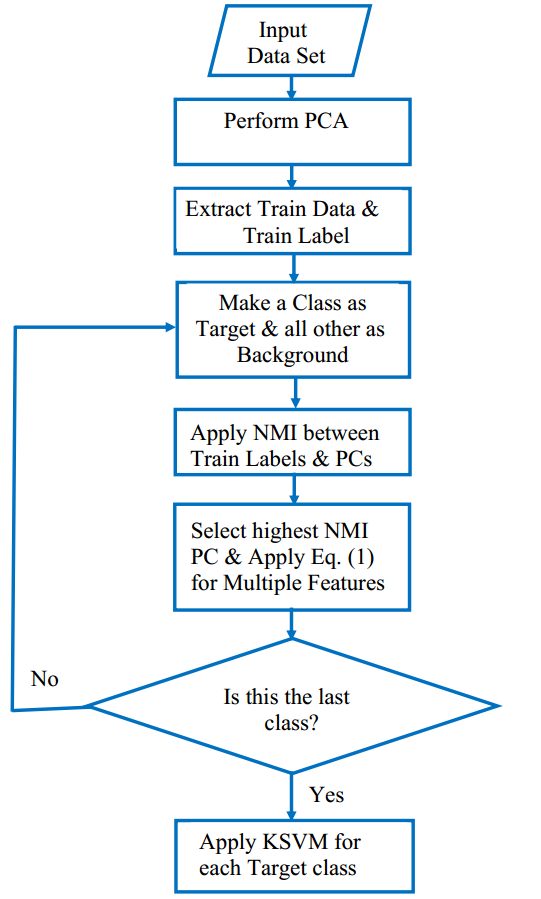
\includegraphics[width=1\linewidth, height = 7.7cm, keepaspectratio]{flow.png}
	\captionof{figure}{Proposed method}
\end{center}

Remote sensing is the acquisition of information about an object or phenomenon without making physical contact with the object and thus in contrast to on-site observation. Remote sensing is used in numerous fields, including geography, land surveying and most Earth Science disciplines (for example, hydrology, ecology, oceanography, glaciology, geology); it also has military, intelligence, commercial, economic, planning, and humanitarian applications.\\

In current usage, the term "remote sensing" generally refers to the use of satellite- or aircraft-based sensor technologies to detect and classify objects on Earth, including on the surface and in the atmosphere and oceans, based on propagated signals (e.g. electromagnetic radiation). It may be split into:
\begin{itemize}\compresslist	
	\item Active remote sensing
	\item Passive remote sensing
\end{itemize}

\begin{center}
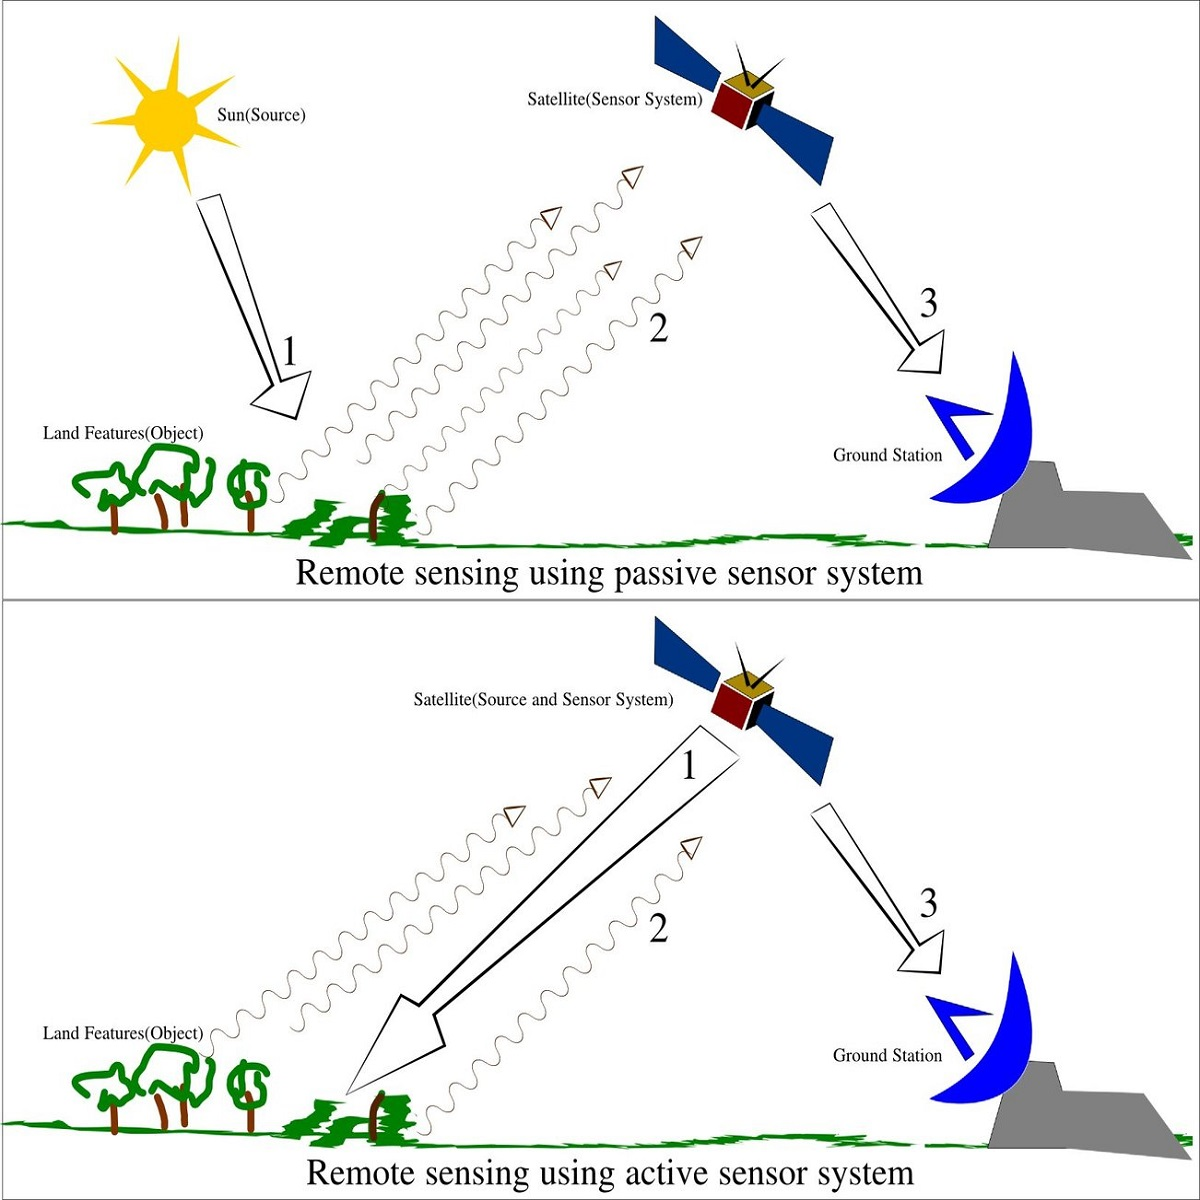
\includegraphics[width=1\linewidth]{Remote_Sensing_Illustration.png}
\captionof{figure}{Remote Sensing Illustration}
\end{center}
\fi

\end{multicols}

}

%----------------------------------------------------------------------------------------
%	REFERENCES
%----------------------------------------------------------------------------------------

\headerbox{References}{name=references,column=0,span=2,above=bottom}{

\renewcommand{\section}[2]{\vskip 0.05em} % Get rid of the default "References" section title
\nocite{*} % Insert publications even if they are not cited in the poster
\small{ % Reduce the font size in this block
\bibliographystyle{unsrt}
\bibliography{sample} % Use sample.bib as the bibliography file
}}

%----------------------------------------------------------------------------------------
%	FUTURE RESEARCH
%----------------------------------------------------------------------------------------

\headerbox{Future Research}{name=futureresearch,column=2,aligned=references,above=bottom}{ % This block is as tall as the references block

This method needs some further improvement to handle the complex class relationships where only a few feature may not capable to complete the task.

}

%----------------------------------------------------------------------------------------
%	CONTACT INFORMATION
%----------------------------------------------------------------------------------------

\headerbox{Contact Information}{name=contact,column=3,aligned=references,above=bottom}{ % This block is as tall as the references block

\begin{description}\compresslist
\item[Web] tanvirtomal.blogspot.com
\item[Email] tanvirahmed14@gmail.com
\item[Phone] +8801753684839
\end{description}
}

%----------------------------------------------------------------------------------------
%	CONCLUSION
%----------------------------------------------------------------------------------------

\headerbox{Conclusion}{name=conclusion,column=2,span=2,row=0,below=results,above=references}{

\begin{multicols}{2}

\begin{center}
	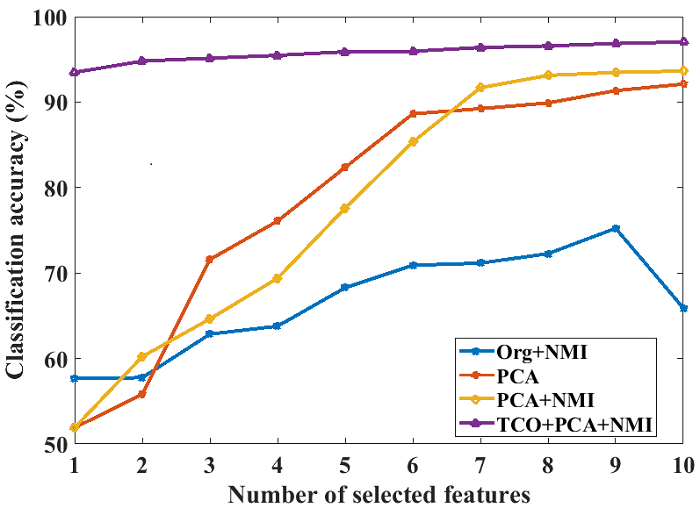
\includegraphics[width=1\linewidth]{Res.png}
	\captionof{figure}{Classification result of AVIRIS 92AV3C}
\end{center}

%------------------------------------------------

\begin{itemize}\compresslist
\item It is clear that the proposed method is able to identify a better subspace which can offer the best classification accuracy among the standard approaches examined.
\item This is because the proposed method selects the most relevant subset of images for required classes.
\end{itemize}

\begin{center}
	\begin{tabular}{|c|c|}
		\hline
		Method & Classification Result\\ \hline
		Org+NMI & 72.26\%\\ \hline
		PCA & 89.90\%\\ \hline
		PCA+NMI & 93.12\%\\ \hline
		TCOSD& 96.57\%\\ \hline
	\end{tabular}
\captionof{table}{Classification result for 8 features}
\end{center}

\end{multicols}
}

%----------------------------------------------------------------------------------------
%	PROPOSED METHOD
%----------------------------------------------------------------------------------------

\headerbox{Proposed Method}{name=method,column=0,below=objectives,bottomaligned=conclusion}{ % This block's bottom aligns with the bottom of the conclusion block

The Proposed method is summarised as follows:
\begin{enumerate}\compresslist
\item Perform PCA and generate new features
\item Extract the training data and training label
\item Consider one class as target at a time, i.e, make a class as target and all other class as background. 
\item Apply NMI between the training labels and the principal components.
\item Select the best principal component based on the high value of NMI. List the selected subset. 
\item Apply the Eq. (1) for selecting multiple features based on NMI for the target class.
\item Apply the selected features to the KSVM classifier.
\item Repeat step 3 to 6 by making another class as target and the remaining as background.
\end{enumerate}

\begin{equation}
	\hat{R}(\textbf{Y}_i,k) = \hat{I}(\textbf{Y}_i,\textbf{C}) - \dfrac{1}{k} \sum_{\textbf{Y} = S_k} \hat{I}(\textbf{Y}_i,\textbf{Y}),  \textbf{Y}_i\notin S_k
\end{equation}

We call this method as Target Class Oriented Subspace Detection (TCOSD).

}

%----------------------------------------------------------------------------------------
%	RESULTS 2
%----------------------------------------------------------------------------------------

\headerbox{Results}{name=results2,column=1,below=objectives,bottomaligned=conclusion}{ % This block's bottom aligns with the bottom of the conclusion block

\begin{center}
	\begin{tabular}{|c|c|c|}
		\hline
		Method & C & $\gamma$ \\ \hline
		Org+NMI & 10 & 2.44 \\ \hline
		PCA & 19 & 2.40 \\ \hline
		PCA+NMI & 16 & 0.7\\ \hline
		TCOSD & 5 & 0.75\\ \hline
	\end{tabular}
\captionof{table}{Details of parameter for KSVM(RBF kernel)}
\end{center}

\begin{center}
	\begin{tabular}{|c|l|}
		\hline
		Target class & Order of selected features\\ \hline
		Hay-windrowed & PC: 4,1,17,5,12,3,16,2\\ \hline
		Soybean-notil & PC: 1,17,16,11,20,14,13,3\\ \hline
		Woods & PC: 1,16,17,3,15,11,5,20\\ \hline
		Wheat & PC: 6,19,17,3,12,16,11,5\\ \hline
		Grass/trees & PC: 4,9,5,6,16,17,2,1\\ \hline
		Soybean-min & PC: 1,17,16,3,5,12,11,9\\ \hline
		Corn-min & PC: 1,17,16,5,11,3,20,19\\ \hline
		Stone-steel & PC: 3,4,1,17,16,10,5,11\\ \hline
		Alfalfa & PC: 4,17,15,20,3,16,6,12\\ \hline
		Grass/Pasture & PC: 9,3,17,6,16,11,1,15\\ \hline
		Corn-notill & PC: 1,17,2,16,11,18,20,19\\ \hline
		Soybean-clean & PC: 1,15,17,3,16,20,12,11\\ \hline
		Corn & PC: 1,19,17,16,18,8,11,3\\ \hline
		Bldg-Grass & PC: 15,16,17,3,18,11,19,4\\ \hline
	\end{tabular}
\captionof{table}{Selected features with the proposed method}
\end{center}

}

%----------------------------------------------------------------------------------------

\end{poster}

\end{document}